\section{Results}                        % what the method produced
\label{sec:results}                      % \secref{sec:results}

This section presents the result of the scan merging method of \secref{sec:msis_merging} applied
to the data recorded with the NavScoot~2 in the Fontaine de N\^imes. For every complete scan, the
vertical sonar measurements were used to estimate the conduit wall with a Gaussian process, the
elevation angle of each echo of the horizontal sonar was estimated with its uncertainty, and the
resulting 3D points were added to the vertical sonar points (Algorithm~\ref{alg:msis_merging}). The
results are shown at two scales. \secref{sec:res_merged} gives an overall view of the conduit and
compares three point clouds: the initial point cloud built from the vertical sonar alone, as in
\citet{margaritis2025internship}; the new points recovered from the horizontal sonar; and the merged
point cloud that combines both. \secref{sec:res_zoom} then zooms on one region of the conduit and
shows it with and without the points of the horizontal sonar, to make the local effect of the
merging visible.

% ------------------------------------------------------------------------------
\subsection{Merged point cloud}          % the three clouds of one dive
\label{sec:res_merged}                   % \secref{sec:res_merged}

Figure~\ref{fig:res_merged} shows the three point clouds from the same viewpoint, so that they can be
compared directly. The initial point cloud (a) contains only the vertical sonar measurements: each
rotation of the vertical sonar gives one cross-section of the conduit, so the wall appears as a
sequence of slices along the trajectory. The points of the horizontal sonar (b) are each echo placed
in 3D at its estimated elevation angle; they sample the walls along the direction of travel, between
those slices. The merged point cloud (c) is the union of both sets.
\hint{Comment on what the horizontal sonar adds: number of points, part of the wall covered,
agreement with the vertical sonar points where both overlap.}                  % \secref{sec:res_merged}

Figure~\ref{fig:res_merged} shows the result of the scan merging on the NavScoot~2 data: the
initial point cloud obtained from the vertical sonar only (a), the points recovered from the
horizontal sonar with their estimated elevation angles (b), and the merged point cloud combining
both (c).
\hint{Comment on what the horizontal sonar adds: number of points, part of the wall covered,
agreement with the vertical sonar points where both overlap.}

\begin{figure}[!htb]                     % initial, horizontal and merged clouds
  \centering
  \begin{minipage}[b]{0.32\linewidth}    % (a) vertical sonar only
    \centering
    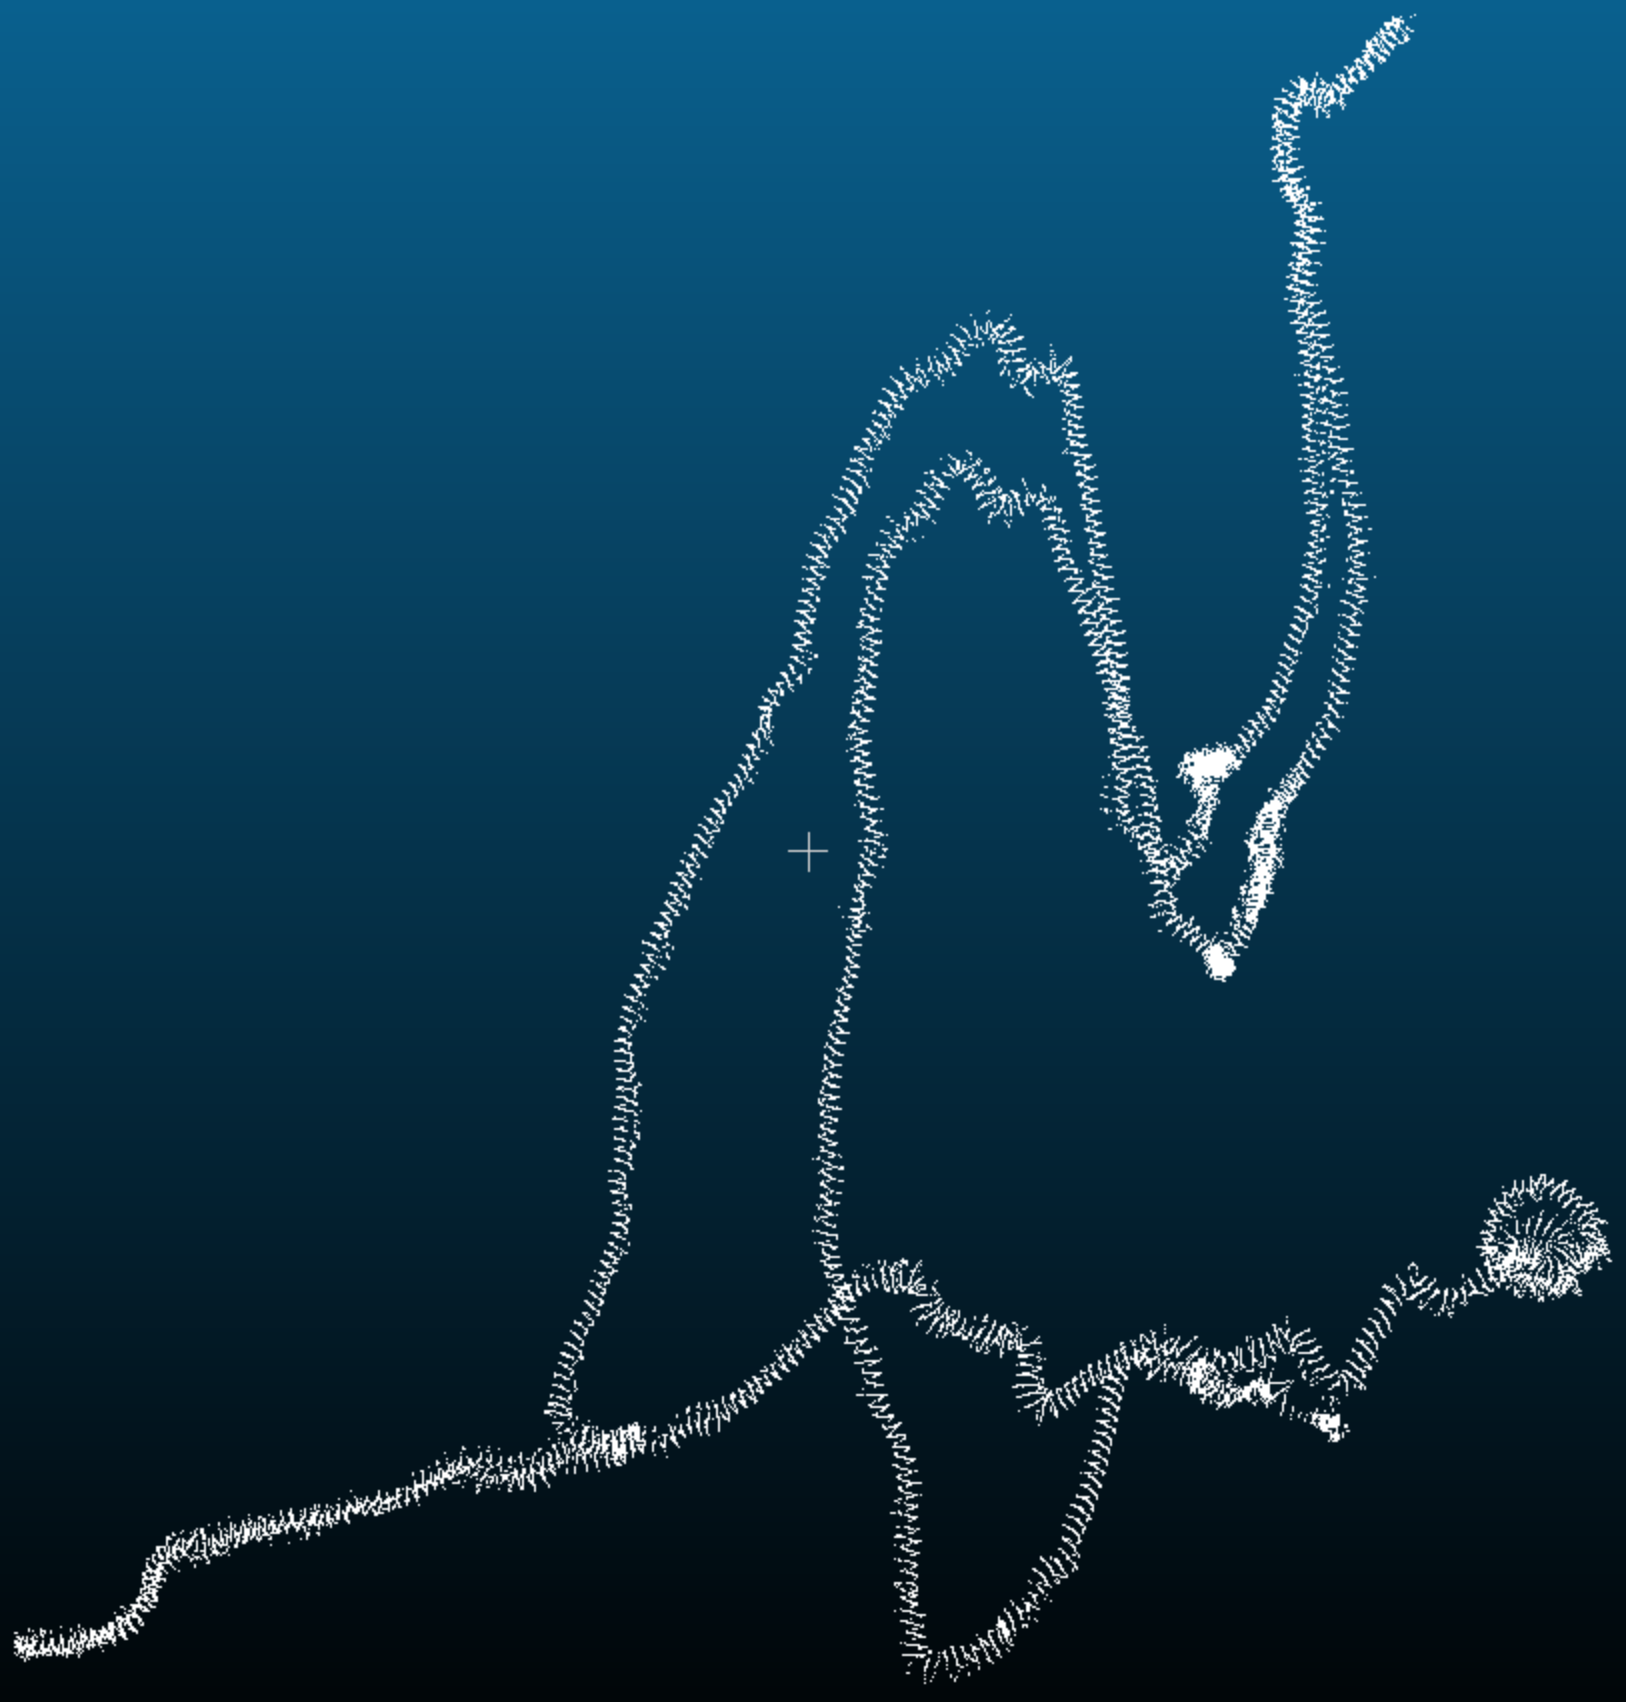
\includegraphics[width=\linewidth, height=4.5cm, keepaspectratio]{figures/RESULT_initial.png}\\[0.2em]
    {\small (a)}
  \end{minipage}\hfill
  \begin{minipage}[b]{0.32\linewidth}    % (b) horizontal sonar points
    \centering
    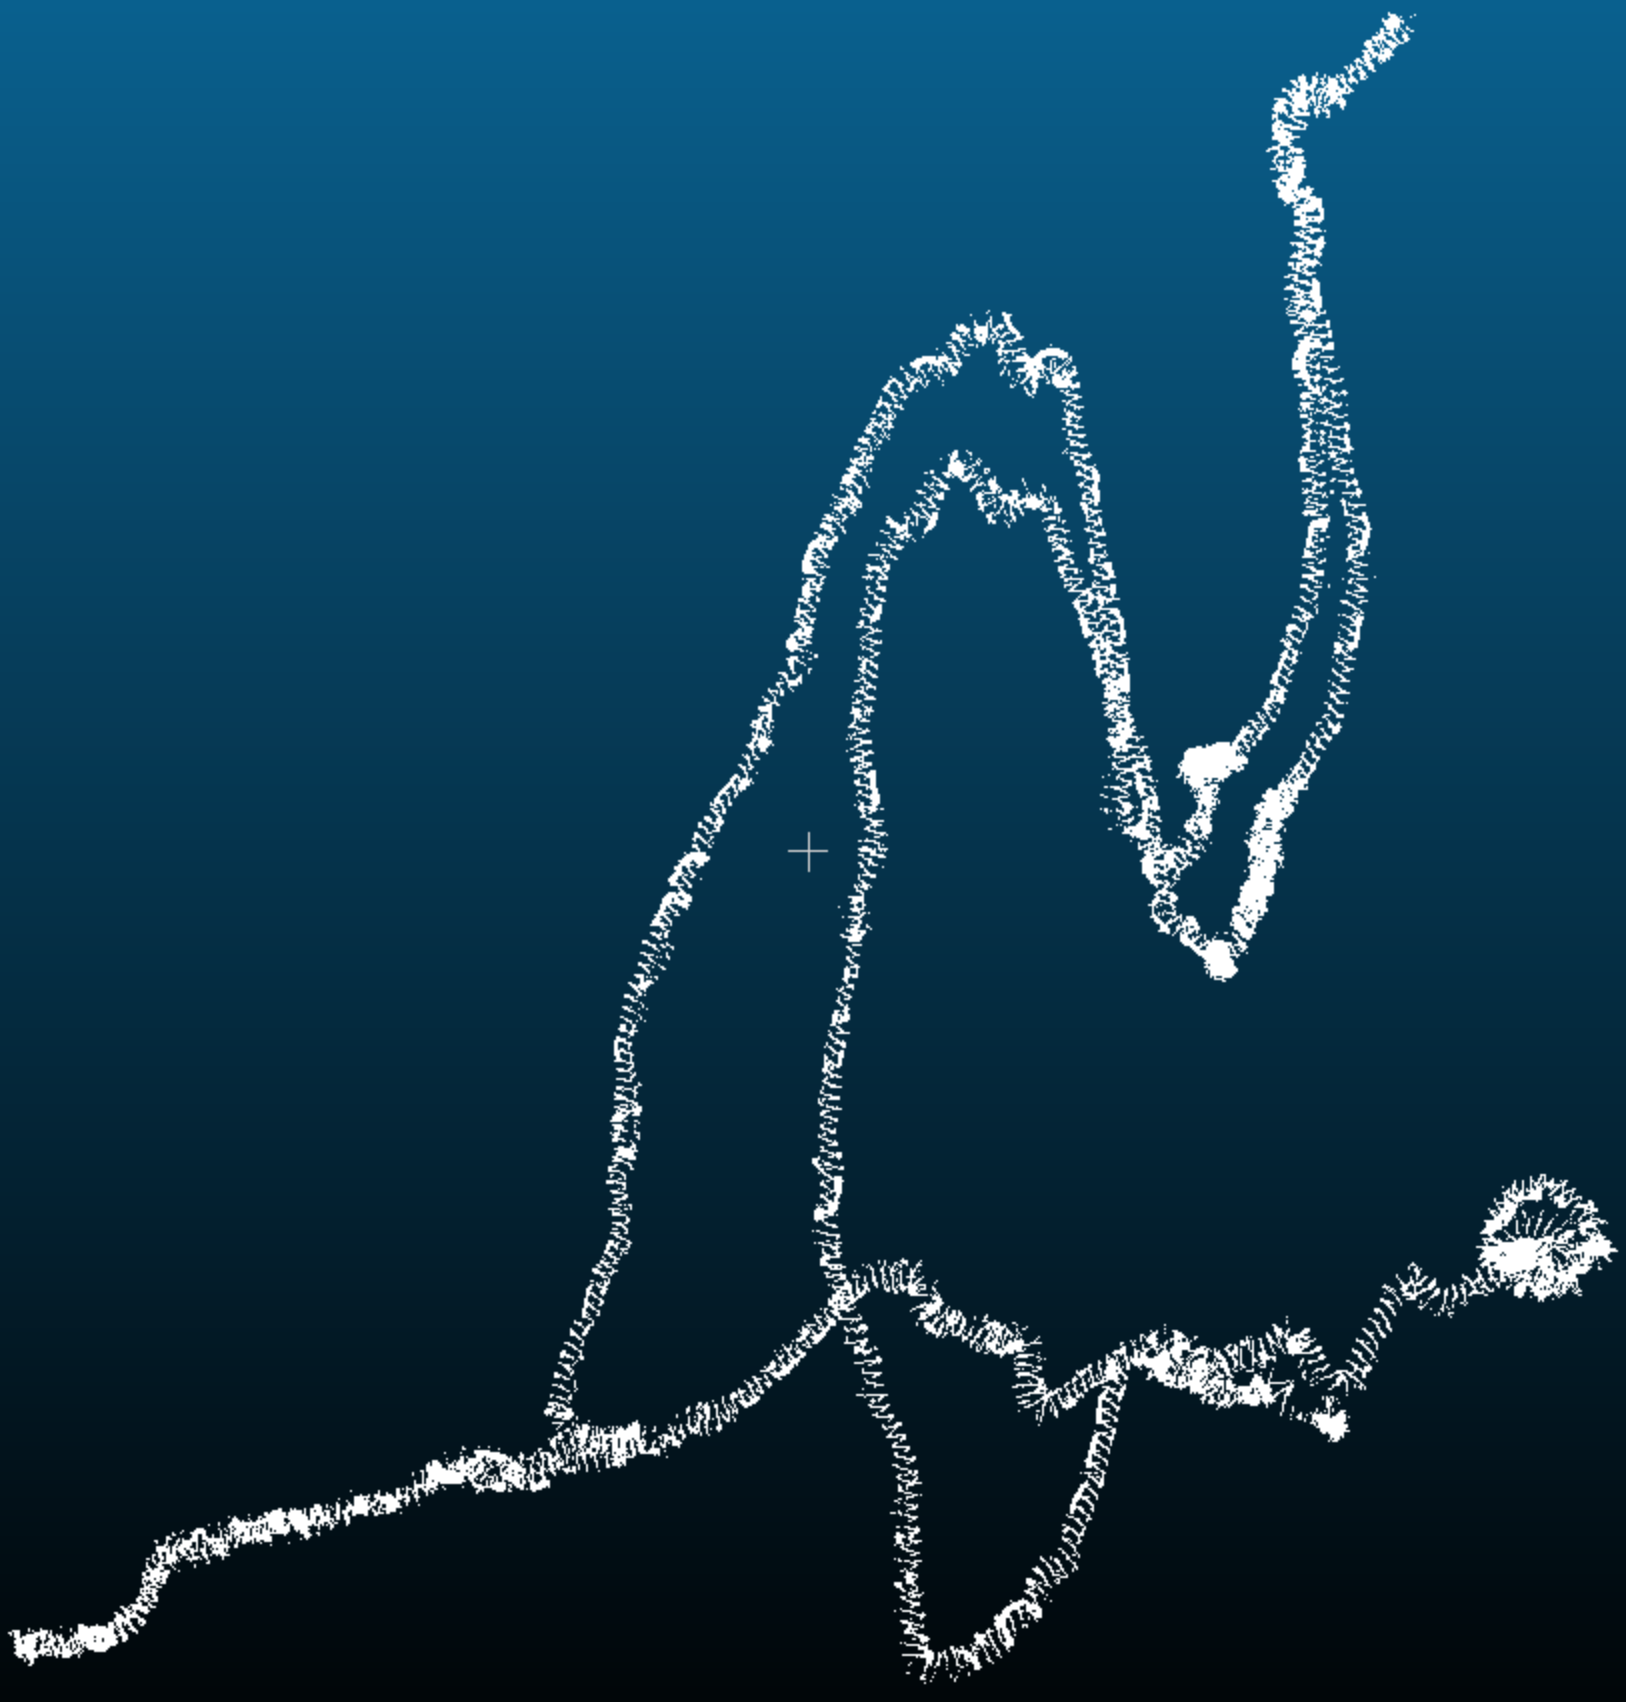
\includegraphics[width=\linewidth, height=4.5cm, keepaspectratio]{figures/RESULT_horizontal.png}\\[0.2em]
    {\small (b)}
  \end{minipage}\hfill
  \begin{minipage}[b]{0.32\linewidth}    % (c) merged cloud
    \centering
    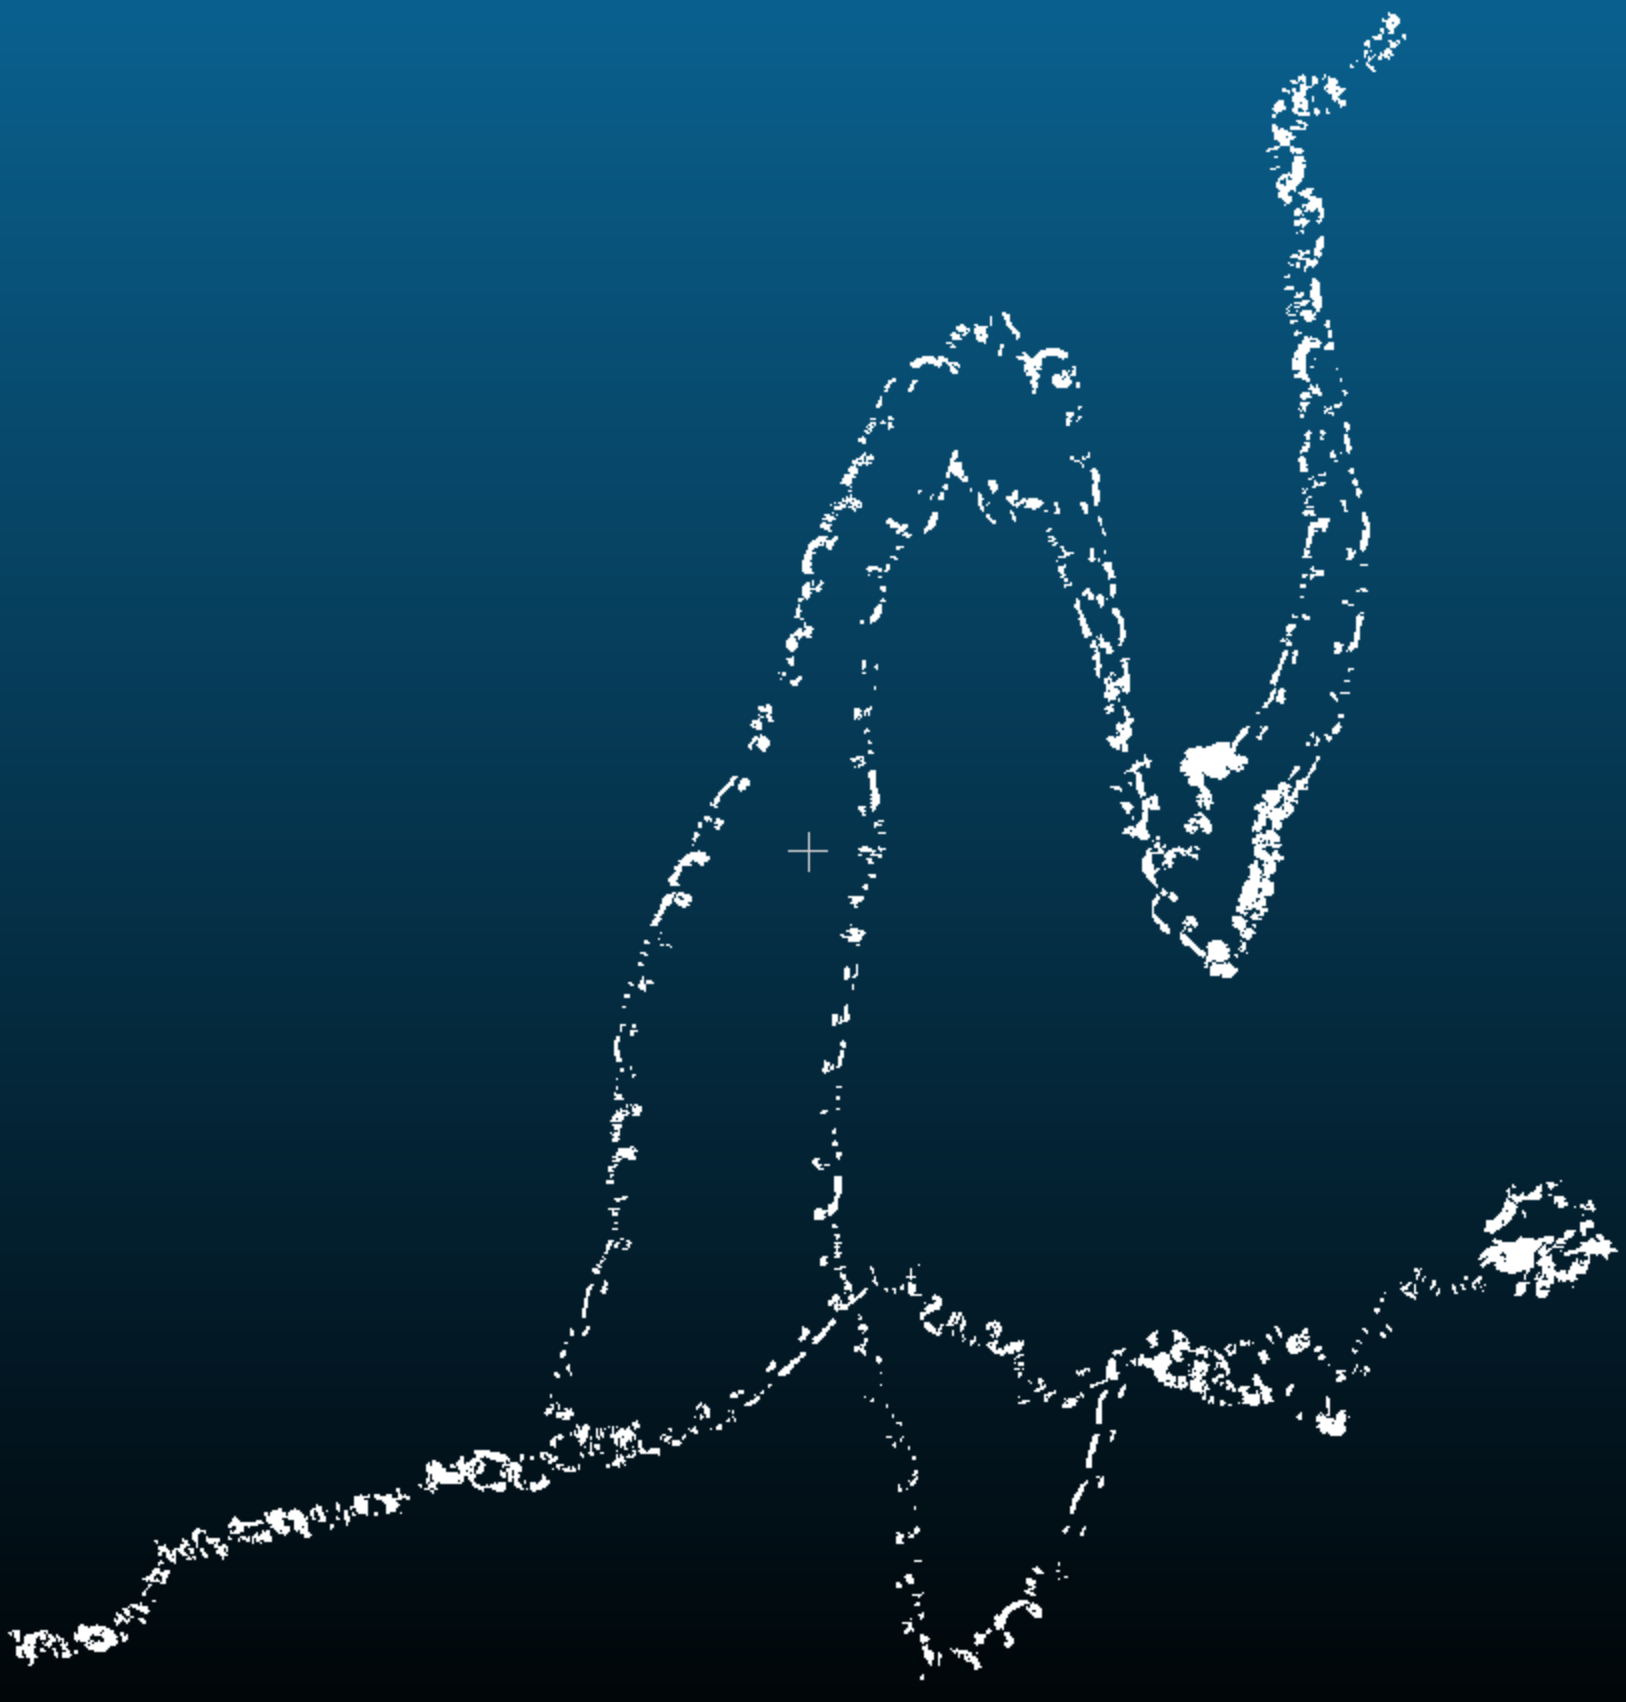
\includegraphics[width=\linewidth, height=4.5cm, keepaspectratio]{figures/RESULT_merged.png}\\[0.2em]
    {\small (c)}
  \end{minipage}
  \caption{Point clouds of the conduit: (a) initial point cloud from the vertical sonar,
           (b) points recovered from the horizontal sonar with the estimated elevation angles,
           (c) merged point cloud.}
  \label{fig:res_merged}
\end{figure}

% ------------------------------------------------------------------------------
\subsection{Close-up comparison}         % local effect of the horizontal sonar
\label{sec:res_zoom}                     % \secref{sec:res_zoom}

At the scale of the whole conduit, the difference between the clouds is hard to judge, so
Figure~\ref{fig:res_zoom} shows a close-up of one region from the same viewpoint, without (a) and
with (b) the points of the horizontal sonar. In (a), the gaps between successive cross-sections of
the vertical sonar are visible; (b) shows how the horizontal points fill these gaps.
\hint{Comment on the local effect: how well the gaps are filled, and any region where the
horizontal points add noise.}                   % \secref{sec:res_zoom}

Figure~\ref{fig:res_zoom} compares the same region of the conduit without (a) and with (b) the
points of the horizontal sonar.
\hint{Comment on the local effect: gaps between the vertical cross-sections filled by the
horizontal points, and any region where they add noise.}

\begin{figure}[!htb]                     % zoom without / with the horizontal sonar
  \centering
  \begin{minipage}[b]{0.49\linewidth}    % (a) without the horizontal sonar
    \centering
    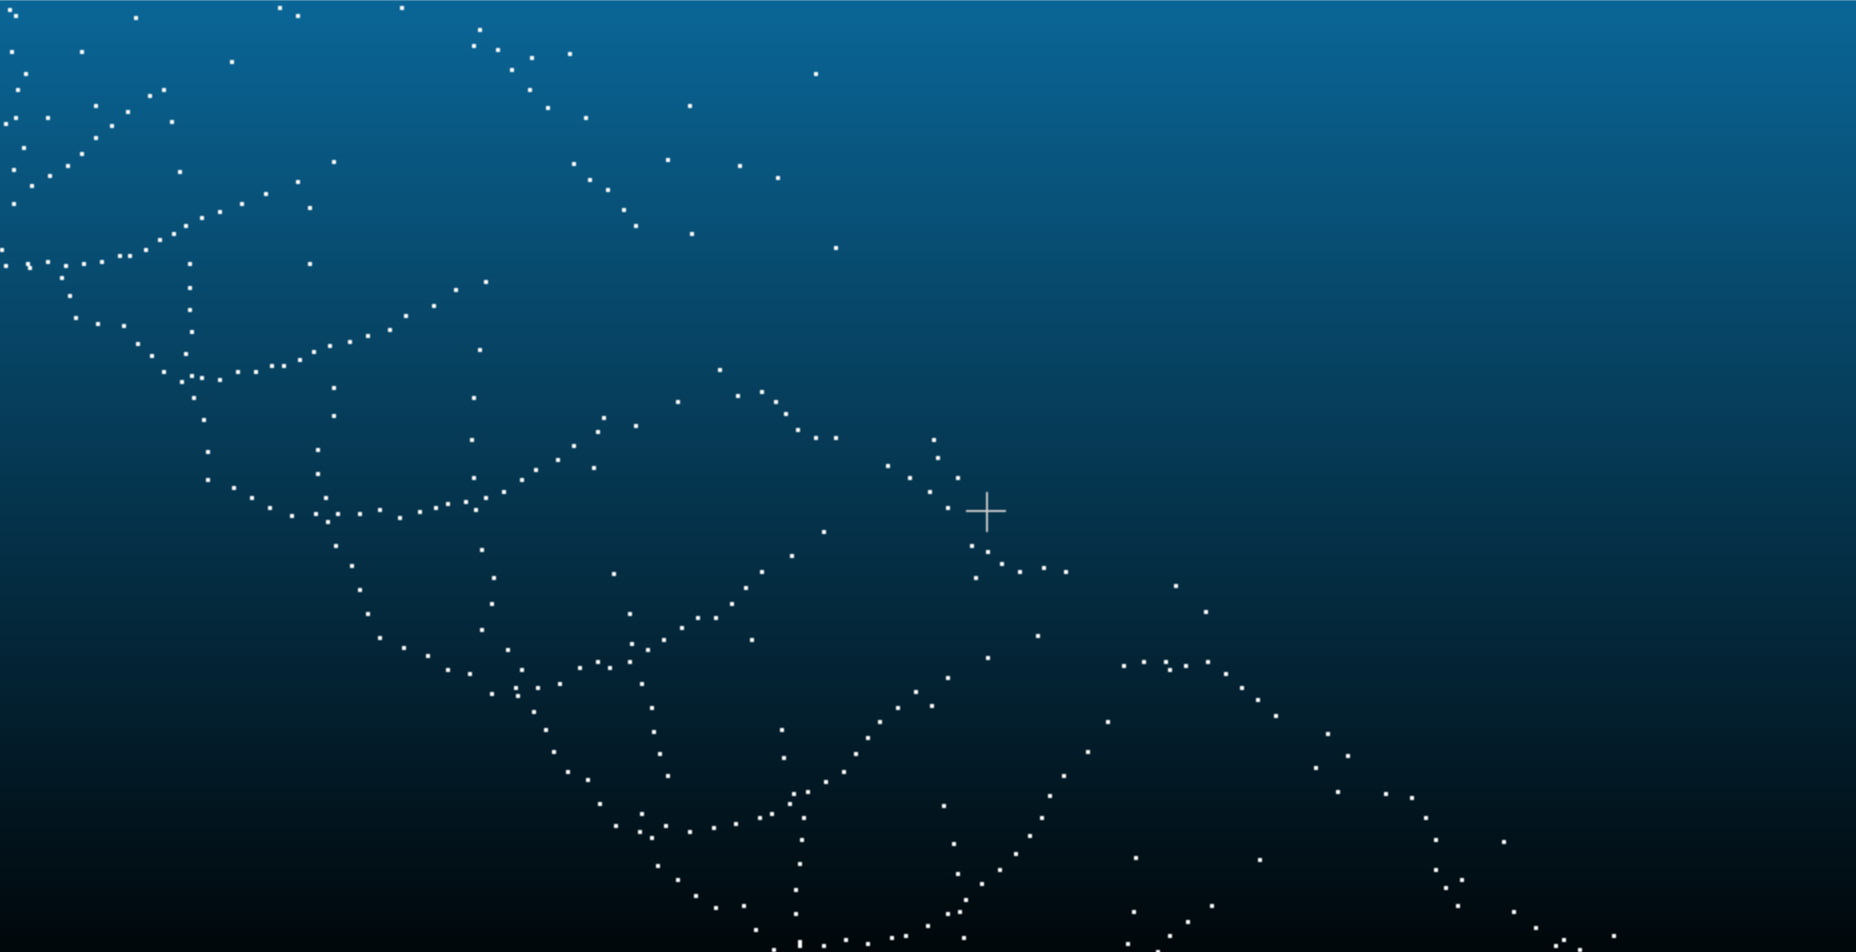
\includegraphics[width=\linewidth, height=6cm, keepaspectratio]{figures/RESULT_zoom_without.png}\\[0.2em]
    {\small (a)}
  \end{minipage}\hfill
  \begin{minipage}[b]{0.49\linewidth}    % (b) with the horizontal sonar
    \centering
    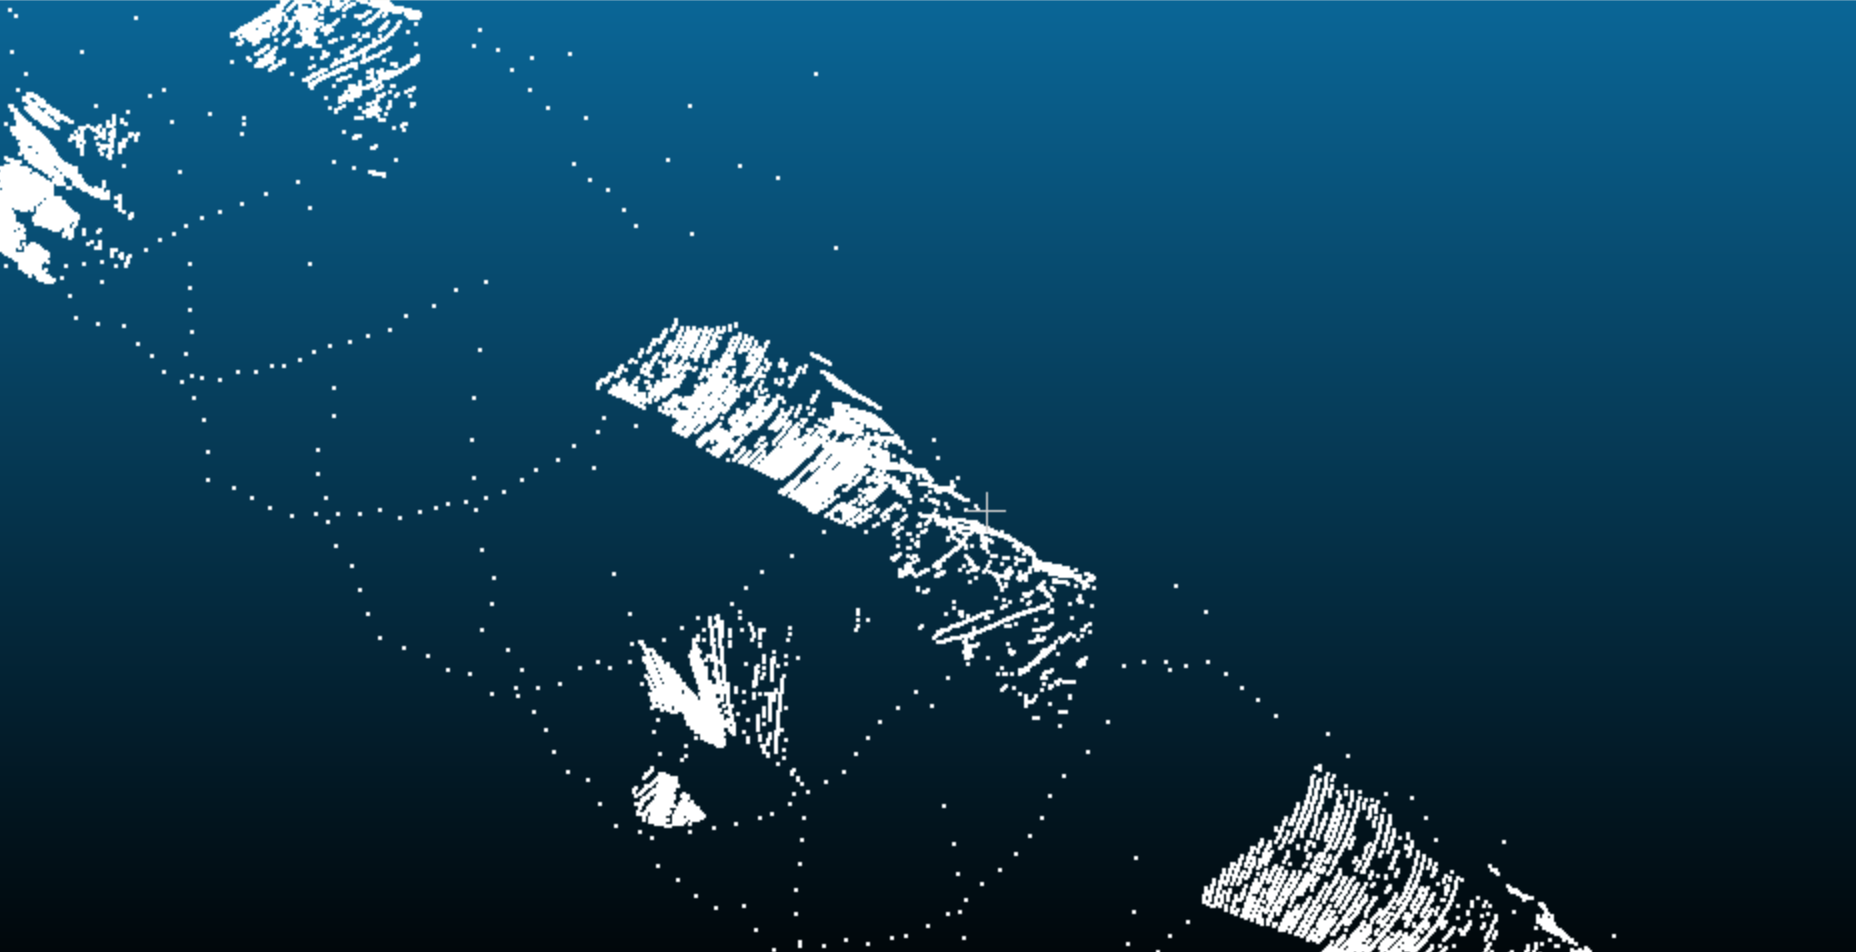
\includegraphics[width=\linewidth, height=6cm, keepaspectratio]{figures/RESULT_zoom_with.png}\\[0.2em]
    {\small (b)}
  \end{minipage}
  \caption{Close-up of the same region of the conduit, (a) without and (b) with the points of the
           horizontal sonar.}
  \label{fig:res_zoom}
\end{figure}